\subsubsection{Spatial Sort}
\label{sec:optim:sort}

\todopfac{THIS}

\begin{figure}[!htp]
	\centering
	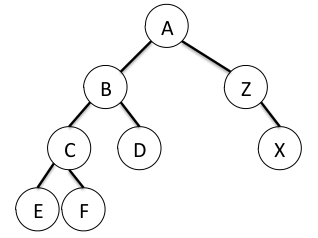
\includegraphics[width=0.4\columnwidth]{pointblocking_tree}
	\caption{A sample tree}
	\label{fig:tree}
\end{figure}

\begin{figure}[!htp]
	\centering
	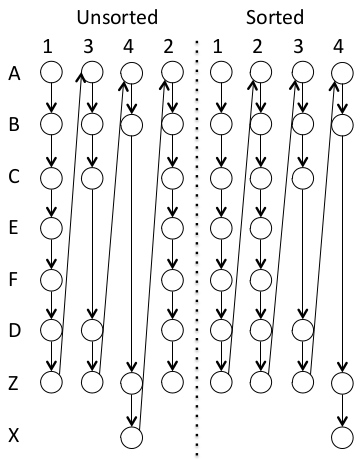
\includegraphics[width=0.6\columnwidth]{pointblocking_sort}
	\caption{Spatial Sort transformation applied to traversal of tree shown in \cref{fig:tree}}
	\label{fig:sort}
\end{figure}

\paragraph{Limitations:}
Processing the points by their geometrical position is only enough with smaller traversal sizes, where the entire traversal fits in cache, and subsequent points, which are likely to follow similar paths due to being geometrically close, will benefit from locality.

But for a sufficiently large traversal, the first visited nodes will have been evicted from cache at the end of the traversal, and when starting the next traversal, will have to be fetched again, increasing misses. \cite{tree_tiler} already shows that, as the traversao size increases, the locality improvements gained from the spatial sort optimization decrease drastically.